\documentclass[type=dr, dr=rernat, accentcolor=tud7b,colorbacktitle, bigchapter, openright, twoside, 12pt ]{tudthesis}
%\documentclass[11pt,twoside,a4paper]{article}
\usepackage[english]{babel} 
\usepackage[utf8]{inputenc}
\usepackage{graphicx}
\usepackage{pstricks}
\usepackage{psfrag}
\usepackage{enumerate}
\usepackage{float}
\usepackage{epsfig}
\usepackage{geometry}
\usepackage{subfigure}
\usepackage{rotating}
\usepackage{minitoc}
% \usepackage{dominitoc}
\usepackage{multirow}
\usepackage{listings}
%\usepackage{appendix}
%\usepackage[breaklinks=true]{hyperref}
%\usepackage{breakcites}

%%%% 1 1/2 facher Zeilenabstand:	
\usepackage{setspace}
\onehalfspacing




\begin{document}
\chapter{Intensity modulated particle therapy for multiple targets}
\label{chapter:vmm}
\minitoc

\section{Introduction}

Lung cancer is the leading cause of cancer-related death, with approximately 160 000 deaths in the U.S. in 2014 \cite{Siegel2014}.
More than half of all patients with lung cancer are diagnosed with stage IV non-small cell lung cancer (NSCLC) \cite{Ramalingam2008, Iyengar2014}.
Prognosis for stage IV NSCLC is poor, with only 12 months median survival after first line chemotherapy \cite{Socinski2013}. 

Stereotactic body radiation treatment (SBRT) shows good results for treating NSCLC \cite{Baumann2009, Fakiris2009, Grutters2010, Greco2011}. 
Furthermore, several studies have shown that SBRT can be used in the setting of limited metastatic 
disease \cite{Rusthoven2009, Villaruz2012, Salama2012, Iyengar2014}. 
Passive scattering particle therapy has also prooved as an effective treatment for NSCLC \cite{Grutters2010, Tsujii2012} and it could be considered an alternative
to photon treatment.

It was shown in Chapter~\ref{PatStudy} that scanned carbon ions (PT) could also be used as a treatment modality for NSCLC. One of the conclusions of the study shown in Chapter~\ref{PatStudy} 
was that patients with multiple disease sites would especially benefit from PT compared to SBRT. However, limitations of this study were the small number of patients (4) and
a single-field uniform optimization (SFUD) used in treatment planning. Multiple disease sites usually occupy a large volume of the lung and hence present themselves in a complex geometry. 
It is not possible to create clinically acceptable treatment plans with SFUD for such complex geometry.

We hypothesise that intensity modulated particle therapy (IMPT), should result in an adequate treatment plans. Furthermore, IMPT 
should provide single fraction scheme in patients, where SBRT due to the OAR dose limitations could not. 

Treatment of lung cancer patients  with multiple disease sites was investigated with state of the art 4D IMPT optimization. 
Treatment plans were generated with two different 4D optimization techniques and compared with SBRT plans, which were actually used for treating patients.


%A simple geometrical union of target contour in different CT states, geo-ITV, leads to poor 4D dose distribution, when treating moving tumors with particle therapy \cite{Rietzel2010}.
\newpage
\section{Materials and Methods}

The 4D extension of GSI's treatment planning system TRiP98 \cite{Kraemer2000a, Richter2013} was used and modified to create treatment plans. A description of modifications and tools used will be given here, 
alongside with patient data.

\subsection{Patient data}


In this study, 8 patients with 2 - 5 lung metastases summing to 24 metastases in total were included. The lesion size was 4.2 cm$^3$ (median, 25-75\% 2.4 - 22.2) and peak-to-peak motion was 5.9 mm (2.7 - 8.1). 
Details are given in Table~\ref{tab:patdata2}.
Target motion and PT treatment planning were based on a 4D-CT, consisting of 10 phases (0 - 9), with phase 0 (end-inhale) chosen as a reference phase.
A registered positron emission tomography (PET) scan was used to delineate clinical target volumes (CTV). 

Patients 1 - 3 had no while patients 4 - 8 had at least one OAR in CTV vicinity (closer than 10 mm).

Patients were treated with SBRT at Chamaplimaud Center for the Unknown, Lisbon (Portugal), with different fraction schemes. 
Number of fractions and doses delivered are given in Table~\ref{tab:patdata2}.

\newpage


\begin{table}[H]
	\centering
	%   \footnotesize
	\caption{Target characteristics, with CTV volumes, peak-to-peak motions, fractionation schemes and number of fields used for PT treatment planning. Last column 
	shows an OAR in target vicinity (closer than 10 mm), if present. SA stands for smaller airways and esoph. for esophagus.}
	\begin{tabular}{c|c|c|c|c|c|c}
		\hline\hline
		\multirow{2}{*}{Patient} & \multirow{2}{*}{Target} & \multirow{2}{*}{Volume (cm$^3$)} & Peak-to-peak & Fractination & Number & OAR in \\
		 & & & motion [mm] & scheme & of fields & proximity \\
		\hline
		\multirow{2}{*}{1} & a & 10.2 & 3.4  & 1 x 24 Gy & 2 & \\
		 & b & 14.4 & 2.8 & 1 x 24 Gy  & 2 &  \\

		 
		 \hline
		 \multirow{5}{*}{2} & a & 3.8 & 5.8  & 1 x 24 Gy & 2 &\\
		  & b & 4.3 & 0.8  & 1 x 24 Gy& 2 &\\
		  & c & 2.7 & 3.4  & 1 x 24 Gy & 2&\\
		  & d & 3.1 & 2.1  & 1 x 24 Gy & 2&\\
		  & e & 0.5 & 0.5  & 1 x 24 Gy & 2&\\
		  \hline
		  \multirow{2}{*}{3} & a & 139 & 0.6 & 1 x 24 Gy & 3 \\
		 & b & 9.2 & 2.0  & 1 x 24 Gy & 2 \\
		 \hline
		 \multirow{2}{*}{4} & a & 4 & 9  & 3 x 9 Gy  & 5 & SA, esoph., heart \\
		 & b & 0.8 & 7.8  & 1 x 24 Gy & 2 \\
		 \hline
		 \multirow{4}{*}{5} & a & 3.4   & 5  & 1 x 24 Gy & 3 &  \\
				    & b & 2.4 & 4.4  & 1 x 24 Gy & 2 &\\
				    & c & 2.0 & 6.3  & 1 x 24 Gy& 2& Heart\\
				    & d & 2.4 & 6.4  & 1 x 24 Gy & 2 & Heart\\
		\hline	    
		\multirow{2}{*}{6} & a & 20.6 & 7.4 & 1 x 24 Gy & 4 & SA  \\
		 & b & 27.1 & 6.0  & 1 x 24 Gy &5 & SA  \\
		 
		 \hline
		 \multirow{2}{*}{7} & a & 2.3 & 12  & 1 x 24 Gy & 2 &\\
		 & \multirow{2}{*}{b} & \multirow{2}{*}{0.4} & \multirow{2}{*}{11.8}  & \multirow{2}{*}{5 x 7 Gy} & \multirow{2}{*}{5} & Heart, esoph., \\
		 & & & & & & stomach \\
		 \hline
		 \multirow{5}{*}{8} & a & 136 & 12  & 3 x 9 Gy & 2 & Heart\\
		  & b & 12.4 & 2.5  & 1 x 20 Gy & 2 &\\
		  & c & 123 & 14  & 3 x 9 Gy & 2  &Heart \\
		 & d & 80.7 & 17  & 1 x 22 Gy & 3  &\\
		 & e & 86.7 & 6.6  & 1 x 20 Gy & 3 & SA \\
		\hline\hline
	\end{tabular}
	\label{tab:patdata2}
\end{table}


\newpage

\subsection{Multiple targets}

The TRiP98 optimization works on minimizing the residual of a nonlinear equation system \cite{Kraemer2000a}. The cost function $E(N)$ for particle number $\vec{N}$ is:
\begin{equation}
\label{eq-costFunc}
 E(\vec{N}) = \sum_{i\in T} \left( D_{plan}^{i} - D_{act}^{i}(\vec{N})\right) +  \theta(D_{act}-D_{max})w_{OAR}\sum_{j\in OAR} \left( D_{act}^{i}(\vec{N}) - D_{Max} \right)
\end{equation}

For a CT voxel $i$ and $j$ in target $T$ and OAR, respectively; $ D_{plan}$, $D_{act}$ and $D_{max}$ are the planned, actual and maximum allowed dose, respectively; $\theta$ is a 
Heaviside step function and $w_{OAR}$ is an OAR specific weight.

The $D_{act}(\vec{N})$ is calculated as
\begin{equation}
 D_{act}(\vec{N}) = \sum_{k=1}^n c_{ik}N
\end{equation}

The coefficient $c_{ik}$ gives the dose deposition at voxel $i$ of a pencil beam $k$, 
with $n$ being the number of pencil beams. 

There is no restriction for the number of targets or fields in the minimizing function, so the first part of Eq.~\ref{eq-costFunc} can be expanded to:

\begin{equation}
\label{eq-multiCost}
 E(\vec{N}) = \sum_{T} \sum_{i\in T} \left( D_{plan}^{i} -\sum_{k=1}^n c_{ik}N\right)
\end{equation}

However, the setup of raster points in TRiP98 allowed only one target. It was therefore expanded in a way that a field was designated to a specific target, as displayed in Fig~\ref{Fig:multiTargets}. 
Raster points for each field are created only around the designated target. All fields contribute dose to all voxels in in optimization. Specifically, $k$ in Eq.~\ref{eq-multiCost} runs over all pencil beams. 
Because the optimization function was not changed, 
all TRiP98 4D functionalities could be used, as explained in the next sections.




\newpage


\begin{figure}[H]
	\begin{center}
		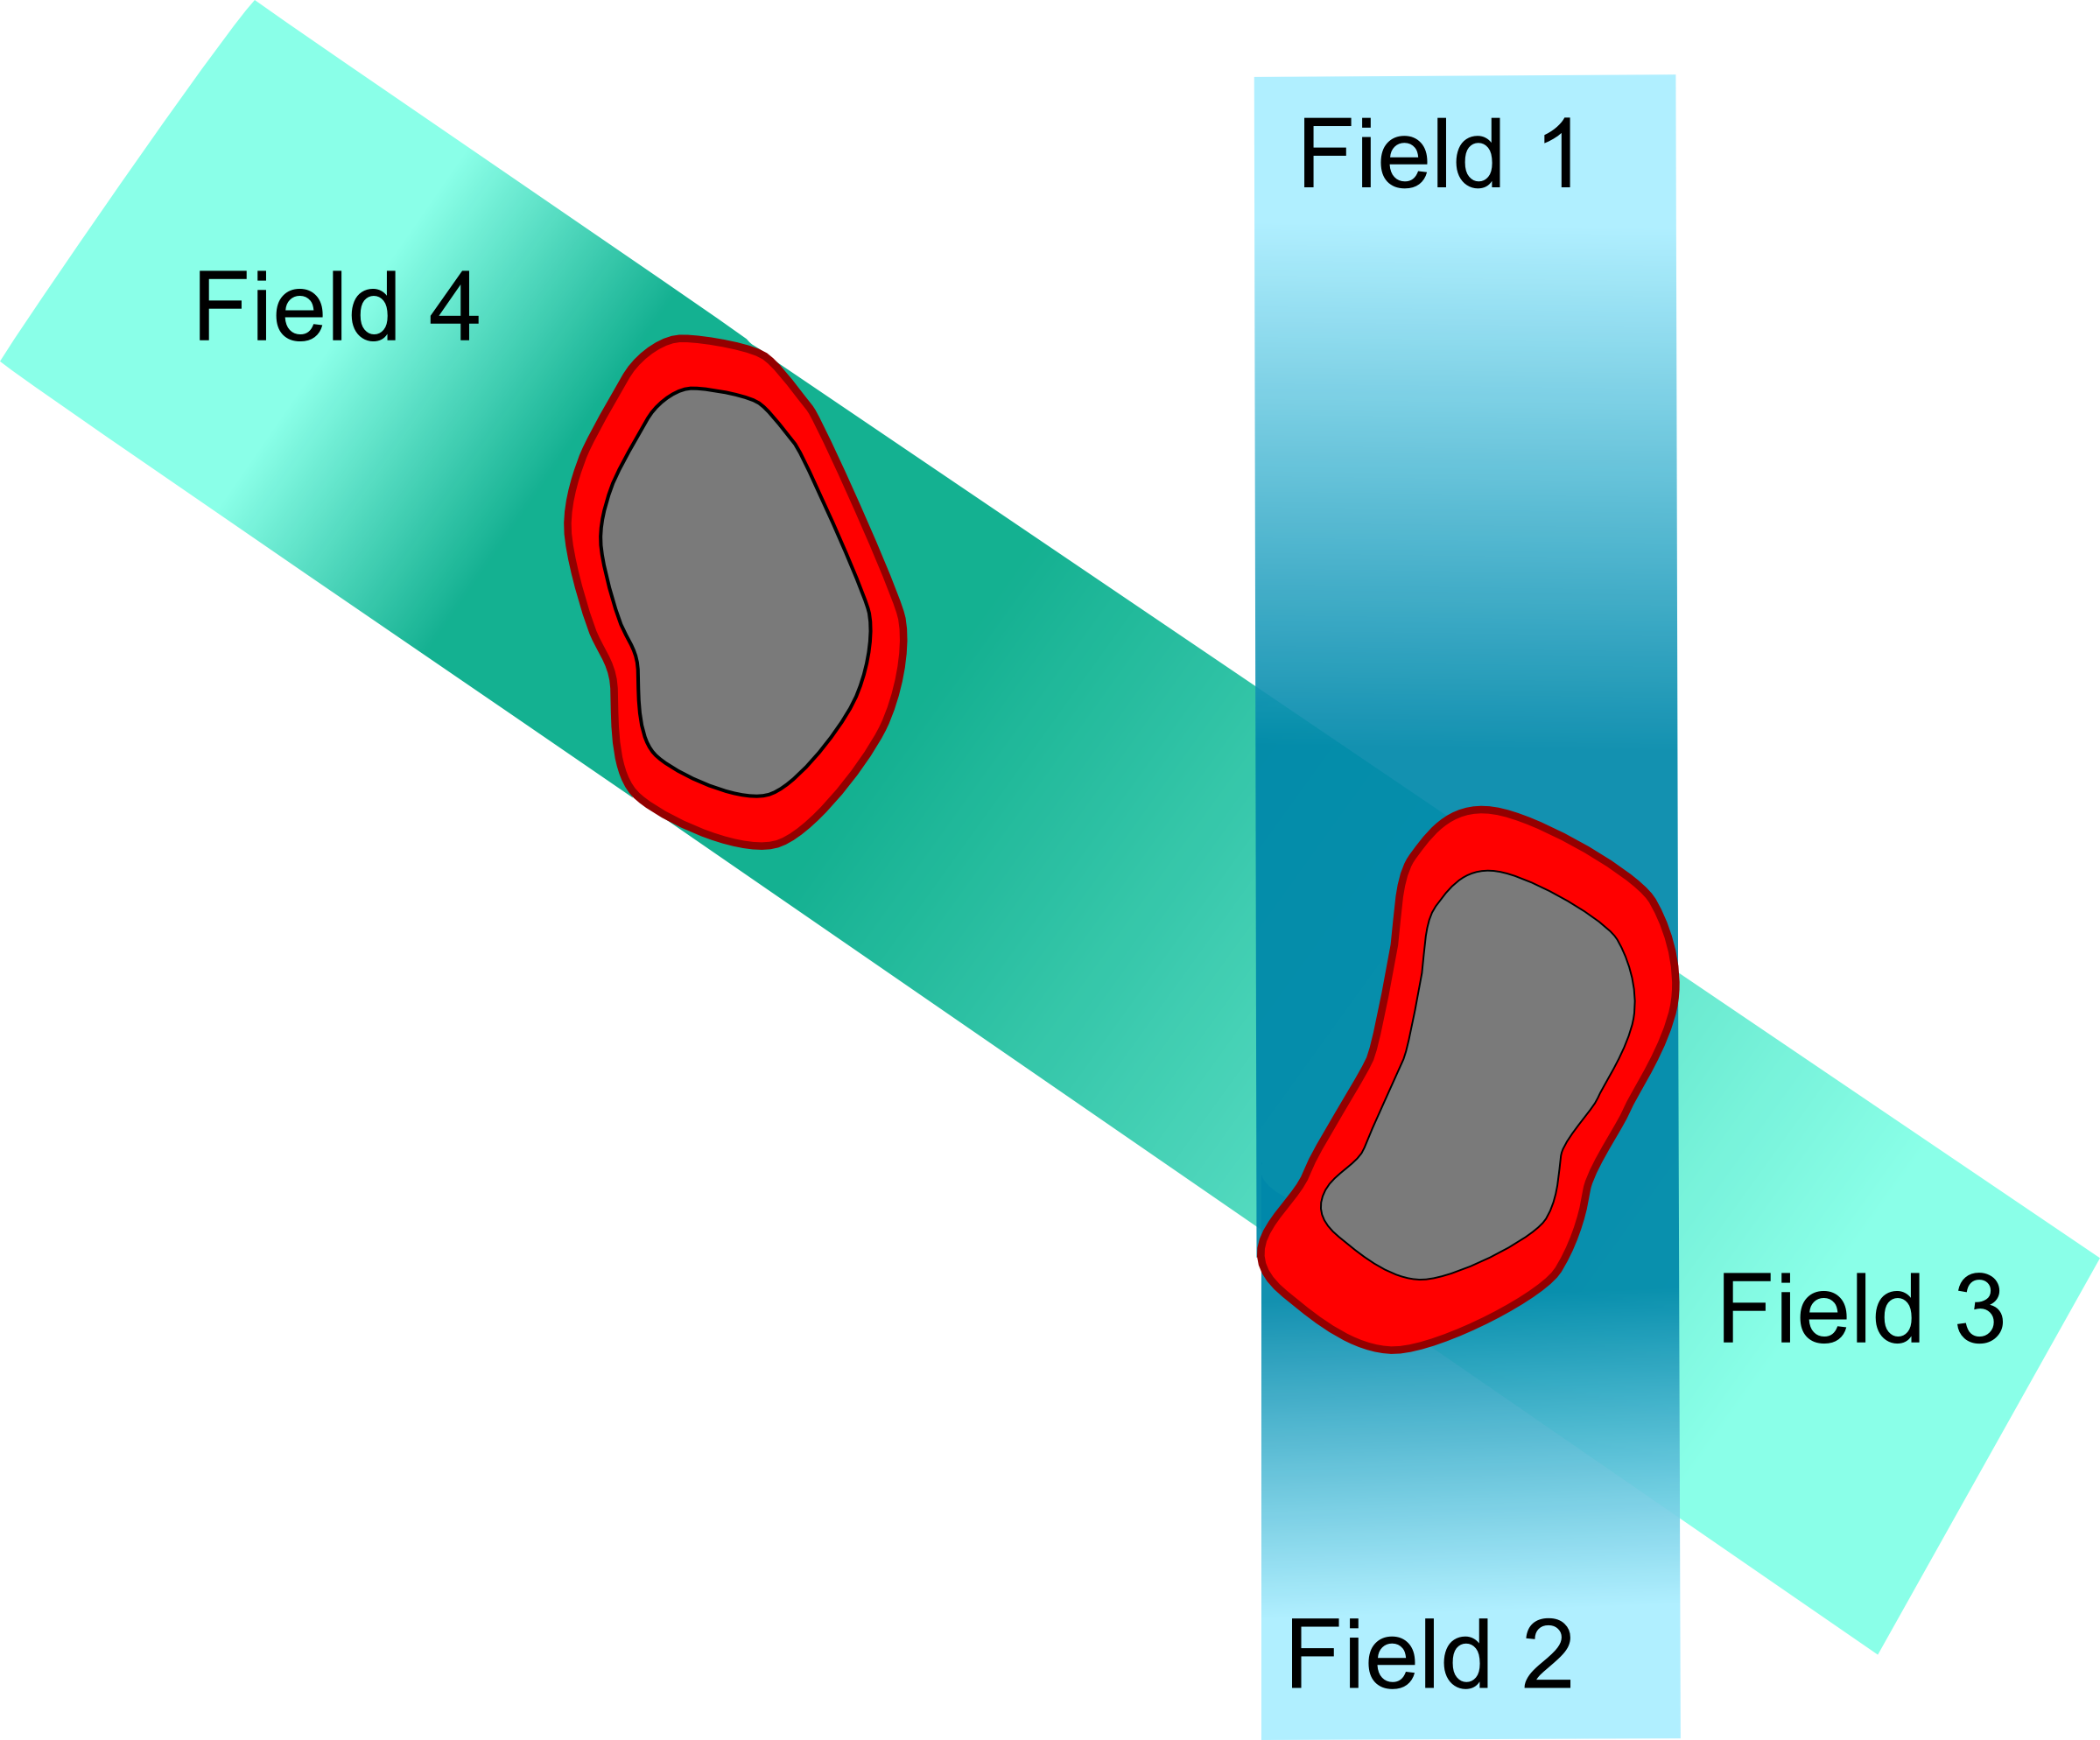
\includegraphics[width=1\textwidth]{./Images/multiTarget.png}
		\caption{Optimization of multiple targets. (a) Fields 1 and 2 are designated to target T1 and fields 3 and 4 to target T2. 
		Optimization takes into account all target voxels and contributions from all fields. An example is shown in (b) and (c), where targets
		were optimized individually (b) and together (c). The dose in (b) reaches almost 200\% in healthy tissue.}
		\label{Fig:multiTargets}
	\end{center}
\end{figure}



\subsection{Optimization techniques}

Investigation of two different optimization techniques to handle range changes in moving tumors was made. For each patient, two sets of plans were created: a field-independent ITV (ITV) and a 4D optimization (4Dopt). 

\begin{itemize}
\item \textbf{Field-independent ITV:} A water-equivalent path length ITV (WEPL-ITV) is different for each field, creating unnecessary margins when combining 
WEPL-ITV from different fields (see Fig.~\ref{Fig:weplITV}a). 
Graeff et. al \cite{Graeff2012} proposed a solution to include range margins into the field description itself, instead of creating a bigger PTV. 

Thus, all fields have the same target in optimization, permiting simultaneous optimization. 
Treatment plans were made for all targets with IMPT on a ITV in reference phase. Additionally target in motion state 5 (end-exhale) was included in optimization
to make plan more robust against range changes in different motion states.

\item \textbf{4D Optimization:} To include WEPL change specific to each motion states a 4D optimization was used. 4Dopt uses a WEPL-ITV for raster setup, 
however the actual optimization is performed on each target voxel in each motion state $m$. The optimization function thus changes to \cite{Graeff2012}:

\begin{equation}
E(\vec{N}) = \sum_{m=1}^{M}\sum_{T_m} \sum_{i\in T_m} \left( D_{plan}^{i} -\sum_{k=1}^n c_{ikm}N\right)
\end{equation}

All targets were treated with IMPT and 4D optimization. Due to the large optimization problem for targets 3a - b, 5a - d, 6b, 8a and 8c, where targets had big volume or 
OARs were included besides targets in optimization a subset of motion states was used \cite{Graeff2012}. 
To cover most of the different tumor positions, two extreme motion states (0 and 5) and an intermidate position (7) were chosen.

\end{itemize}

The same number of fields and the same field angles were used in both techniques.

To reduce optimization problem, only portion of large OARs, such as heart or esophagus, were used. Large OARs were manually cropped to the region close to the 
target. Dose, however, was calculated on a whole OAR to ensure the validty of results.

For targets with different fractionation scheme (targets 8a-e), TRiP98 was modified to include option of specific dose fractions for specific target.


\begin{figure}[H]
	\begin{center}
		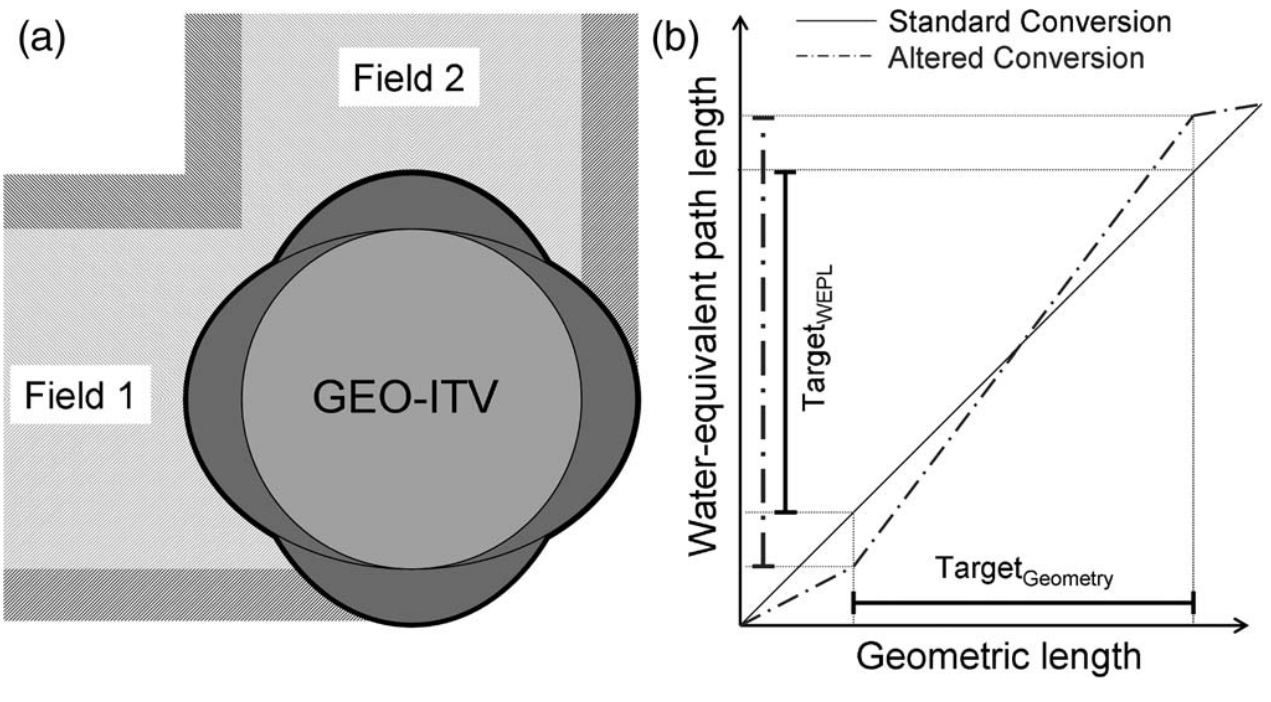
\includegraphics[width=0.7\textwidth]{./Images/weplITV.png}
		\caption{Schematic presentation of the ITV. (a) Dark gray ellipses show margins needed for specific fields to account for range changes in different motion states.
		When common target volume for two perpendicular fields is generated (this black contour) it creates unnecessary lateral extension of both fields, as shown by the dark gray
		entry channels. A solution is shown in (b). Rather than using standard, geometric margins, both fields use the same geometry, however the conversion of geometry to WEPL
		is altered for each field. The plot in (b) shows the standard (solid line) and an altered conversion (dashed-doted line) for a beam passing a homogeneous CTV. The altered conversion
		increases the WEPL extent and thus implicitly increasing margins for a single field only. Figure taken from \cite{Graeff2012}}
		\label{Fig:weplITV}
	\end{center}
\end{figure}

\subsection{Treatment planning}

An isotropic margin of 3 mm was added to each CTV to account for uncertainties in treatment delivery. 
A WEPL-ITV was constructed on the CTV with margins for each individual field, which was than used either in optimization (ITV)
or for raster setup (4Dopt). Due to large memory demands, targets in each lung were optimized separately. 
  
The planning objective was 99\% of each target volume should receive at least 100\% of the planned dose (D$_{99}$\% $\geq$ 100\%). Two dose limitation were used for OARs, as defined in 
the AAPM task group \cite{Benedict2010}. First limitation was a maximum dose to single voxel $D_{Max}$ and second a maximum dose deposited to a 
specific OAR volume $D_{Threshold}$. All limits are summerized in Table~\textbf{appendix}.
 
After the optimization the 4D-dose was calculated for two motion periods (3.6 sec and 5.0 sec) and two starting phases (0$^\circ$ and 90$^\circ$) as explained in Section~\ref{PTTP}. 
The relative biological effectivness (RBE) was calculated with local effect model, LEM IV \cite{Elsaesser2010}. 
Alpha beta ratio of 6 and 2 was used in target and normal tissue, respectively.

Motion was mitigated by applying slice-by-slice rescanning to each plan. 
The number of rescans was limited by the number of particles in a single raster point, which should not be lower than 8000 due to the
monitoring precision. The maximum number of rescanns was limited to 20.

Detailed explanation of SBRT treatment planning is given in Section~\ref{SBRTTP}.

For patients 4 - 7 OAR dose could not be sufficiently reduced in optimization. It was necessary to add margins to the OAR and then 
subtract the OAR plus margins from the target. For SBRT the OAR plus margins was subtracted from PTV, which included 3 mm isotropic margins on geometrical ITV. 
In PT geometrical ITV was not used, so in each of 10 motion states OAR plus margins was subtracted from CTV plus 3 mm. 

Appropriate margins for OAR were found by trial and error. In the first try the OAR was included in optimization with different weights ($w_{OAR}$ in Eq~\ref{eq-costFunc}) and without any substraction from target. 
If any 3D treatment plan after the optimization was acceptable, a 4D dose was calculated, 
where OAR and target dose were inspected. If the plan was rejected, the optimization was repeated but with OAR substraction from target. 
Firstly with no OAR margins and afterwards increasing by 1 mm. 


\subsection{Fraction escalation}

A single fraction of 24 Gy could not be used in SBRT treatment for targets 4a, 7b and 8a-e due to the OAR dose constraints. For these targets additional PT plans were generated with 1 x 24 Gy fractionation scheme, in order
to estimate if PT could respect OAR constraints for these targets, while delivering 1 x 24 Gy. 


\section{Results}

Example of different treatment plans for three patients are shown in Fig.~\ref{Fig:multiExample}. Patient 2 had a 1 x 24 Gy fractionation scheme for 5 targets, without any OARs in CTV vicinity.
Target 7b was in close proximity to the heart, esophagus and stomach and a 5 x 7 Gy fractionation scheme was used to satisfy OAR dose constraints. 
Patient 8 had 5 targets with large total target
volume and target 8a was close to the heart. The heart dose was the limiting factor and hence a complex fractionation scheme was used (see Table~\ref{tab:patdata2}). 
PT was able to deliver 1 x 24 Gy to all targets with only
violating smaller airways and heart $D_{Max}$ by 83\% and 10\%, respectively.

\newpage
\begin{figure}[H]
	\begin{center}
		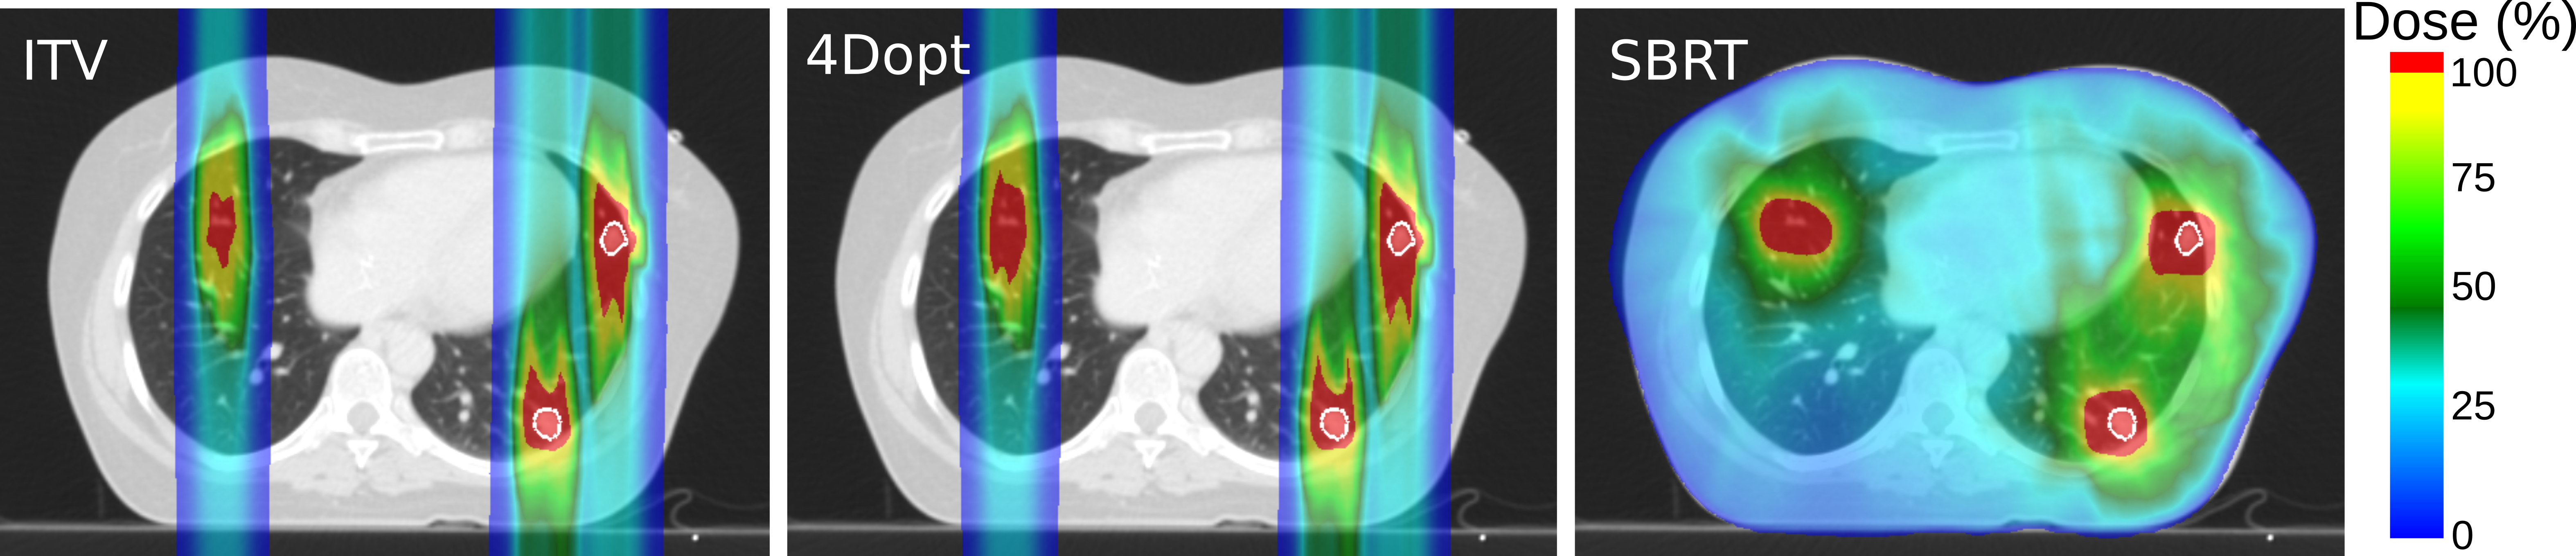
\includegraphics[width=0.9\textwidth]{./Images/multiExample.png}
		\caption{Treatment plans for ITV (left), 4Dopt (middle) and SBRT (right) for patients 2 (top), 7 (middle) and 8 (bottom). 
		CTV, heart, esophagus and stomach contours are outlined in white, red, blue and orange,
		respectively. Patient 7 image is magnified to the target 7b location. Patient 2 has 5 disease sites with no OARs in target vicinity. Patient 7 had poor target coverage
		with PT due to large target motion and OAR proximity. A 1 x 24 Gy plan could be generated for patient 8 with PT, 
		while SBRT was limited with heart dose and 2 targets were treated with 3 x 7 Gy, 2 with 1 x 20 Gy and one with 1 x 22 Gy. }
		\label{Fig:multiExample}
	\end{center}
\end{figure}
\newpage
\subsection{Target Coverage}

Results for CTV $D_{99\%}$ for all patients are shown in Table~\ref{tab:resultsComplex}. All SBRT plans were approved by a physician, 
even though the prescription dose for patients 4 - 6 was not met due to an OAR proximity. Target 7b $D_{99\%}$ for PT was below prescription and SBRT delievered full dose.
Excluding patients 4 - 7, there were 1 and 5 cases (out of 128) of too low CTV dose across different
motion types for ITV and 4Dopt, respectively. For patients 4 - 6 ITV and 4Dopt had higher CTV $D_{99\%}$ than SBRT, except for target 5c and 4a for ITV.
% The lowest CTV $D_{99\%}$ was 75\% for target 7b.

% There was no significant difference in CTV $D_{99\%}$ between SBRT, ITV and 4Dopt.

\begin{table}[H]
	\centering
	%   \footnotesize
	\caption{CTV $D_{99\%}$ for ITV, 4Dopt and SBRT for 8 patients. Results for ITV and 4Dopt are shown as median (range) across different motion types.}
	\begin{tabular}{c|c|c|c|c}
		\hline\hline
		\multirow{2}{*}{Patient} & \multirow{2}{*}{Target} & \multicolumn{3}{|c}{CTV $D_{99\%}$ (\%)}  \\
		 &  & ITV & 4Dopt & SBRT \\
		 \hline9
		 
\multirow{2}{*}{1} & a & 101.0(101.0 - 101.0) & 101.0(101.0 - 101.0) & 100.0\\ 
 & b & 101.0(101.0 - 102.1) & 101.0(101.0 - 101.0) & 100.0\\ 
 \hline
\multirow{5}{*}{2} & a & 101.0(101.0 - 102.1) & 100.0(99.0 - 102.1) & 106.3\\ 
 & b & 102.1(102.1 - 102.1) & 102.1(102.1 - 102.1) & 103.1\\ 
 & c & 101.0(100.0 - 101.0) & 101.6(101.0 - 102.1) & 104.2\\ 
 & d & 102.1(101.0 - 102.1) & 102.1(102.1 - 102.1) & 107.3\\ 
 & e & 101.0(101.0 - 101.0) & 101.0(101.0 - 102.1) & 108.3\\ 
 \hline
\multirow{2}{*}{3} & a & 101.0(101.0 - 101.0) & 101.0(101.0 - 101.0) & 101.0\\ 
 & b & 98.4(97.9 - 99.0) & 98.4(97.9 - 99.0) & 102.1\\ 
 \hline
\multirow{2}{*}{4} & a & 65.3(63.9 - 69.4) & 70.4(68.5 - 72.2) & 66.7\\ 
 & b & 101.0(100.0 - 102.1) & 100.5(100.0 - 102.1) & 103.1\\ 
 \hline
\multirow{4}{*}{5} & a & 100.0(99.0 - 101.0) & 100.0(100.0 - 100.0) & 101.0\\ 
 & b & 101.6(100.0 - 102.1) & 97.9(96.9 - 99.0) & 101.0\\ 
 & c & 95.3(94.8 - 96.9) & 94.3(92.7 - 94.8) & 99.0\\ 
 & d & 99.0(97.9 - 99.0) & 99.5(99.0 - 100.0) & 94.8\\ 
 \hline
\multirow{2}{*}{6} & a & 89.1(88.5 - 90.6) & 85.4(85.4 - 87.5) & 69.8\\ 
 & b & 78.6(77.1 - 79.2) & 72.4(71.9 - 72.9) & 69.8\\ 
 \hline
\multirow{2}{*}{7} & a & 102.1(102.1 - 102.1) & 99.0(99.0 - 99.0) & 101.0\\ 
 & b & 83.9(82.1 - 85.7) & 75.0(75.0 - 75.0) & 100.0\\ 
 \hline
\multirow{5}{*}{8} & a & 100.0(100.0 - 100.9) & 100.0(100.0 - 100.9) & 105.6\\ 
 & b & 101.3(100.0 - 102.5) & 101.3(100.0 - 102.5) & 105.0\\ 
 & c & 100.0(99.1 - 100.0) & 100.0(99.1 - 100.0) & 106.5\\ 
 & d & 102.3(102.3 - 102.3) & 102.3(102.3 - 102.3) & 102.3\\ 
 & e & 102.5(102.5 - 102.5) & 102.5(102.5 - 102.5) & 101.3\\ 
\hline\hline
	\end{tabular}
	\label{tab:resultsComplex}
\end{table}

\subsection{Dose in OARs}

$D_{Max}$ and $D_{Threshold}$ for 8 OARs are shown in Table~\ref{tab:OARComplex}. Dose volume histograms (DVH) for patients 4, 6 and 7 are shown in Fig.~\ref{Fig:dvh}.
There was a significant difference between PT and SBRT in $D_{Max}$ and $D_{Threshold}$ 
for heart, spinal cord, esophagus and aorta and in $D_{Threshold}$ for smaller airways.
No significant difference was observed in dose to OAR between different motion types or between ITV and 4Dopt.
The overall OAR difference for patients between SBRT and ITV
was significant, 17 (4 - 50)\% and 27 (8 - 56)\% of OAR limits for $D_{Max}$ $D_{Threshold}$, respectivelly. There was no significant difference between ITV and 4DITV to overall dose to OAR.
The ipsilateral lung $V_{20\%}$ was 14.4 (0.0 - 43.0), 14.6 (0.0 - 41.4) and 29.8 (5.8 - 89.2)\% for ITV, 4Dopt and SBRT, respectively. Both, ITV and 4DITV ipsilateral lung $V_{20\%}$ was
significantely different from SBRT, while no significant difference was observed between ITV and 4DITV.

The margins used for OAR subtraction for PT and SBRT, respectively, were:
2 and 5 mm for smaller airways, 0 and 1 mm for esophagus in patient 4; 
0 and 2 mm for heart in patient 5; 
2 and 11 mm for smaller airways in left lung, 0 and 9 mm for smaller airways in right lung in patient 6;
2 and 0 mm for esophagus and 0 and 1 mm for stomach in patient 7.

All treatment plans exceeded the $D_{Max}$ limit for smaller airways in patients 4, 6 and 8 and for heart in patient 6. 
Additionally, SBRT Esophagus and Heart $D_{Max}$ limits were exceeded in patients 4 and 8, respectively.


\begin{table}[H]
	\centering
	%   \footnotesize
	\caption{OAR $D_{Max}$, $D_{Threshold}$ and ipsilateral lung $V_{20\%}$ of all patients for ITV, 4Dopt and SBRT. There was a significant difference between PT and SBRT for all OARs, except
	smaller airways' $D_{Max}$. $D_{Max}$ and $D_{Threshold}$ doses are normalized to the corresponding OAR limits in the fractionation scheme used (see \cite{Benedict2010}). 
	Data is displayed as median (range).}
	\begin{tabular}{c|c|c|c}
		\hline\hline
		 
		OAR &  ITV & 4Dopt & SBRT \\
		\hline
		& \multicolumn{3}{c}{$D_{Max}$ (\%)}  \\
		\hline
heart & 63.0(0.0 - 95.0) & 37.0(0.0 - 97.0) & 82.5(20.0 - 103.0)\\ 
spinalcord & 3.0(0.0 - 59.0) & 1.5(0.0 - 61.0) & 60.0(21.0 - 79.0)\\ 
smallerairways & 60.0(0.0 - 126.0) & 25.0(0.0 - 130.0) & 72.5(0.0 - 171.0)\\ 
esophagus & 4.0(0.0 - 91.0) & 4.0(0.0 - 21.0) & 70.5(20.0 - 101.0)\\ 
aorta & 10.5(0.0 - 63.0) & 13.5(0.0 - 63.0) & 45.0(15.0 - 74.0)\\
\hline\hline
& \multicolumn{3}{c}{$D_{Threshold}$ (\%)} \\
\hline
heart & 14.0(0.0 - 66.0) & 8.5(0.0 - 56.0) & 62.5(19.0 - 98.0)\\ 
spinalcord & 2.0(0.0 - 53.0) & 0.0(0.0 - 60.0) & 66.5(28.0 - 95.0)\\ 
smallerairways & 28.5(0.0 - 91.0) & 1.5(0.0 - 91.0) & 68.5(0.0 - 99.0)\\ 
esophagus & 0.0(0.0 - 16.0) & 0.0(0.0 - 4.0) & 49.0(17.0 - 99.0)\\ 
aorta & 3.5(0.0 - 30.0) & 2.5(0.0 - 24.0) & 34.5(12.0 - 59.0)\\ 
\hline\hline
& \multicolumn{3}{c}{$V_{20\%}$ (\%)} \\
\hline
ipsilateral lung & 14.4(0.0 - 43.0) & 14.6(0.0 - 41.4) & 29.2(0.0 - 89.2)\\
\hline\hline
	\end{tabular}
	\label{tab:OARComplex}
\end{table}

% \begin{table}[H]
% 	\centering
% 	%   \footnotesize
% 	\caption{$D_{Max}$ and $D_{Threshold}$ for OAR in CTV vicinity for ITV, 4Dopt and SBRT. The rightmost column shown allowed doses,
% 	as defined in \cite{Benedict2010}.}
% 	\begin{tabular}{c|c|c|c|c}
% 		\hline\hline
% 
%  \multicolumn{5}{c}{Patient 1} \\ 
% SmallerAirways & 20.6(20.5 - 21.0) & 24.8(24.5 - 25.0) & 17.5& 13.3\\ 
% Esophagus & 23.0(22.3 - 23.5) & 23.3(23.0 - 23.5) & 25.5& 15.4\\ 
% Heart & 28.0(28.0 - 28.3) & 28.1(28.0 - 28.5) & 29.3& 22\\ 
%  \multicolumn{5}{c}{Patient 4} \\ 
% Heart & 22.8(22.3 - 23.3) & 23.1(22.0 - 24.3) & 22.8& 22\\ 
%  \multicolumn{5}{c}{Patient 5} \\ 
% AirwaysSmallR & 18.4(17.5 - 19.0) & 18.8(18.5 - 19.0) & 15.3& 0\\ 
% AirwaysSmallL & 22.5(21.8 - 23.3) & 18.0(17.8 - 18.3) & 25.5& 0\\ 
%  \multicolumn{5}{c}{Patient 7} \\ 
% SmallerAirways & 21.3(21.0 - 21.8) & 20.3(19.8 - 20.3) & 16.0& 13.3\\ 
% Heart & 29.8(29.5 - 30.0) & 29.5(29.3 - 29.5) & 30.5& 22\\ 
% 
% \hline\hline
% 	\end{tabular}
% 	\label{tab:OARComplex}
% \end{table}

\newpage
\begin{figure}[H]
	\begin{center}
		\includegraphics[width=0.9\textwidth]{./Images/DVH_legend.png}
		\caption{Dose volume histograms for targets 4b, 6a, 6b and 7b with relevant OARs. SBRT, ITV and 4DITV are represented by solid, dashed and dotted line, respectively. Targets are displayed
		in grayscale, while OAR colors are shown in legend. SA stands for smaller airways.}
		\label{Fig:dvh}
	\end{center}
\end{figure}
\newpage


\subsection{Fractination escalation}

With PT the 1 x 24 Gy fractionation scheme could be used for targets 8a-e, violating only $D_{Max}$ for smaller airways (180\%) and heart (110\%). 
SBRT for patient 8 was limited by heart $D_{Threshold}$ which was 100\% of the allowed dose - for PT it was 45\% in the same fractionation scheme.

For targets 4a and 7b the 1 x 24 Gy frascionation scheme could not be generated with PT. Either the target coverage was low (CTV $D_{99\% < 50\%}$) or 
esophagus $D_{Max}$ and additionally stomach $D_{Max}$ for target 7b were exceeded.

\section{Summary and Discussion}

Clinically valid SBRT plans have been compared to PT treatment plans for NSCLC patients with multiple metastases. 
To the best of our knowledge, this is the first study of treating multiple NSCLC metastases with IMPT. A novel approach was used to handle multiple targets and combined
with state of the are 4D IMPT treatment planning. Furthermore, 4D PT doses were calculated for different motion types. 

PT on average delivered less dose to OARs, while still having comparable target coverage to SBRT.
The most important difference is in heart dose, with $D_{Threshold}$ being on average 6 times lower in PT compared to SBRT. Recent trial has shown,
that a higher heart dose could be attributed to higher mortality rates for NSCLC patients \cite{Bradley2015}.

For patients with complex geometry (4 - 8) PT maintained or even improved target coverage in most cases, while reducing doses to OARs.
The exception was target 7b, where CTV $D_{99\%}$ was low (84\% and 75\% for ITV and 4Dopt, respectivelly), due to the $D_{Max}$ constraints of esophagus and stomach.
The large motion of target 7b (11.8 mm) and small target volume (0.4 cm$^3$) contributed to a poor PT plan, whereas SBRT was able to deliever full dose to the target
and adhearing to OAR constraints. This supports our claim in Chapter~\ref{PatStudy} that targets with larger volume would benefit most from PT. Furthermore, for small targets
with large motion in a OAR vicinity, PT generates worse plan than SBRT. It should be noted, however, that integral doses for all OARs are still lower for PT as seen in Fig~\ref{Fig:dvh}.
The only limitation for PT are usually the OAR's $D_{Max}$.

Due to the OAR constraints of targets 4a and 7b, no fractionation escalation was possible with PT. 
For patient 8, however, the fractionation scheme could be changed to 1 x 24 Gy. Large total target volume could be irradiated with less
overall dose to the patient and hence significantely reducing the heart dose. Again, this confirms our claim of PT benefit for large targets.


There was no significant difference between ITV and 4Dopt in target coverage or in dose to OAR. 
However, in patients 4 and 6 the 4Dopt was able to achieve better target coverage. With ITV, target 4a had worse coverage than 4Dopt and delievered more high dose to 
smaller airways (see Fig~\ref{Fig:dvh}. For patient 6, 4Dopt deposited less dose to smaller airways in addition to better target coverage.


Even though PT deposits less dose to OARs with the same or even better target coverage, there is still room for improvement in PT 4D treatment planning. 
An implementation of multi-criteria objective planning should bring even better dose distribution and bring possibility to choose between trade-offs \cite{Breedveld2007, Chen2010}. 
Additionally, multiple target optimization in PT would benefit from a shell around PT where dose would be minimized. Therefore excessive dose
in healthy tissue would be further reduced. An introduction of a shell, however, would further enlarge the optimization problem, which is big already for complex geomteries (patient 4 - 8). 
A possible solution to minimize the voxel number in optimization would be an adaptive dose grid \cite{Prall2016a}.

In Chapter~\ref{PatStudy} additional range margins to account for range uncertainties could be used in treatment planning, due to SFUD. 
Because we did not use field specific PTVs it was not possible to include range uncertainties in our study.
Instead of creating field specific PTVs to include range uncertainties, a solution was proposed to include uncertainties in optimization process itself \cite{Pflugfelder2008, Unkelbach2009, Fredriksson2011, Chen2012}.
Chen et al. have shown it is possible to implement robust optimization in multi-criteria optimization as well \cite{Chen2012}. Furthermore, in a recent treatment planning study by Liu et al. \cite{Liu2016}
a 4D robust optimization was demonstrated, with better results over 3D robust optimization for NSCLC patients. However, only breathing starting phase was used as an uncertainty,
whereas different motion types should be considered. The disadvantage of 3D and 4D robust optimization is the enlargement of the optimization problem.

Patient 6 $D_{Max}$ heart dose ranged over 2 Gy across different motion types in 4Dopt, showing the necessity of making treatment plans robust against motion uncertainty, 
especially in the hypo-fractionated regiment. Furthermore, OAR doses that are under the limits after optimization, may exceed them after calculating 4D dose. 
The ITV and 4Dopt approaches take into account range changes in different motion states, however they do not address interplay. 
This could be solved with a complete 4D optimization \cite{Graeff2013}, where a 4D raster treatment plan is 
generated and each motion state has a designated treatment plan. 

% Clinical application of beam tracking is not yet feasible due to several reasons, such as the 
% inverse interplay, the ion-beam tracking system complexity, precision and speed of the motion monitoring.
% Another solution would be jet-ventilation \cite{Santiago2013}, however, it brings additional complications to treatment.

Apart from 4D robust optimization, the effect of motion could be minimized by using other motion mitigation techniques, such as gating. Furthermore, gating could improve the target coverage, where the planned dose was
not met. Gating, together with rescanning, has already been successfully implemented clinically for active beam scanning \cite{Rossi2016, Mori2016} and it might be essential to use it in hypo-fractionated 
treatment of moving tumors \cite{Richter2014}.

A recent review showed good local control rates between 66 - 92\% for patients treated with SBRT for in-rield recurrent tumors \cite{Amini2014}. 
However, there were grade 4 and 5 complications present, i.e. study by Trovo et al showed grade 5 pneumonia in
6\% of patient treated \cite{Trovo2014}. As shown in our study, PT delivers less dose to the OAR, ipsilateral lung in particular, and could hence reduce the number of treatment-related
complications.

\section{Conclusions}

PT delivers less dose to OAR compared to SBRT in NSCLC patients with multiple disease sites, while maintaining target coverage. Patient with large total target volume 
could be irradiated with 1 x 24 Gy, whereas it could not with SBRT. For a small target with large motion and OARs in vicinity, 
SBRT generated better treatment plan. 
No significant difference was found between two 4D optimization techniques. However, 4D optimization showed better results for some patients with OAR in CTV vicinity.


\bibliographystyle{apalike}
\bibliography{../ref.bib}{}
% \bibliographystyle{plain}

\end{document}